\documentclass[border=12pt]{standalone}
\usepackage{pgfplots}
\pgfplotsset{compat=1.8}

\begin{document}
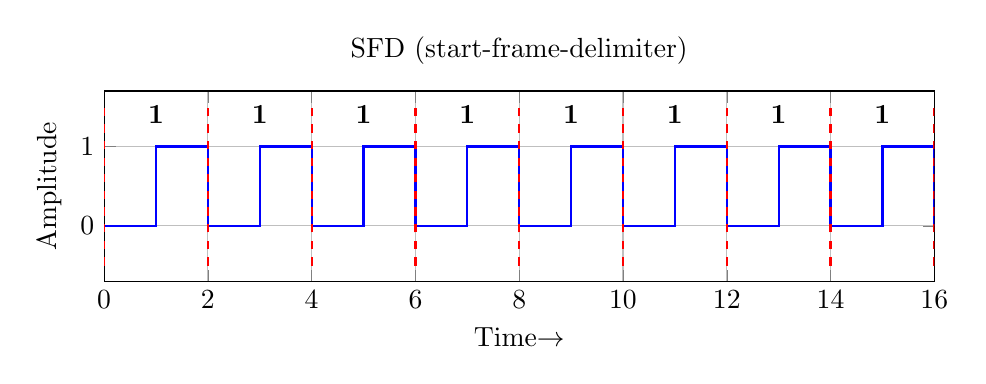
\begin{tikzpicture}
    \begin{axis}[grid=both,xmin=0,xmax=16,width=\textwidth,height=4cm,
        title=SFD (start-frame-delimiter),xlabel={Time$\rightarrow$},ylabel=Amplitude]
        \addplot+[thick,blue,const plot, no marks,samples at={0,1,...,16}] {(mod(x,2)>0?1:0)};
        \pgfplotsinvokeforeach{0,...,8} {
            \node[] at (axis cs: #1*2-1,1.40) {\textbf{1}};
            \addplot+[thick,red,dashed,no marks]  coordinates { (#1*2,-0.5) (#1*2,1.5) };
            \pgfmathparse{Mod(#1,2)==0?1:0}
            \ifnum\pgfmathresult>0  
                % \ifnum (mod(#1,2) > 0)
                \addplot+[thick,red,dashed,no marks]  coordinates { (#1,-0.5) (#1,1.5) };
            \fi
        }
    \end{axis}
\end{tikzpicture}
\end{document}
